\documentclass{article}

\usepackage{graphicx}
\usepackage{tikz}
\usepackage{tikzsymbols}
\usetikzlibrary{calc,patterns,shapes.geometric}
\pagestyle{empty}
\usepackage[margin=0pt]{geometry}
\geometry{papersize={14in,12in}}

\def\centerarc[#1](#2)(#3:#4:#5){\draw[#1] ($(#2)+({#5*cos(#3)},{#5*sin(#3)})$) arc (#3:#4:#5);}

\begin{document}
	\begin{figure}
		\centering
		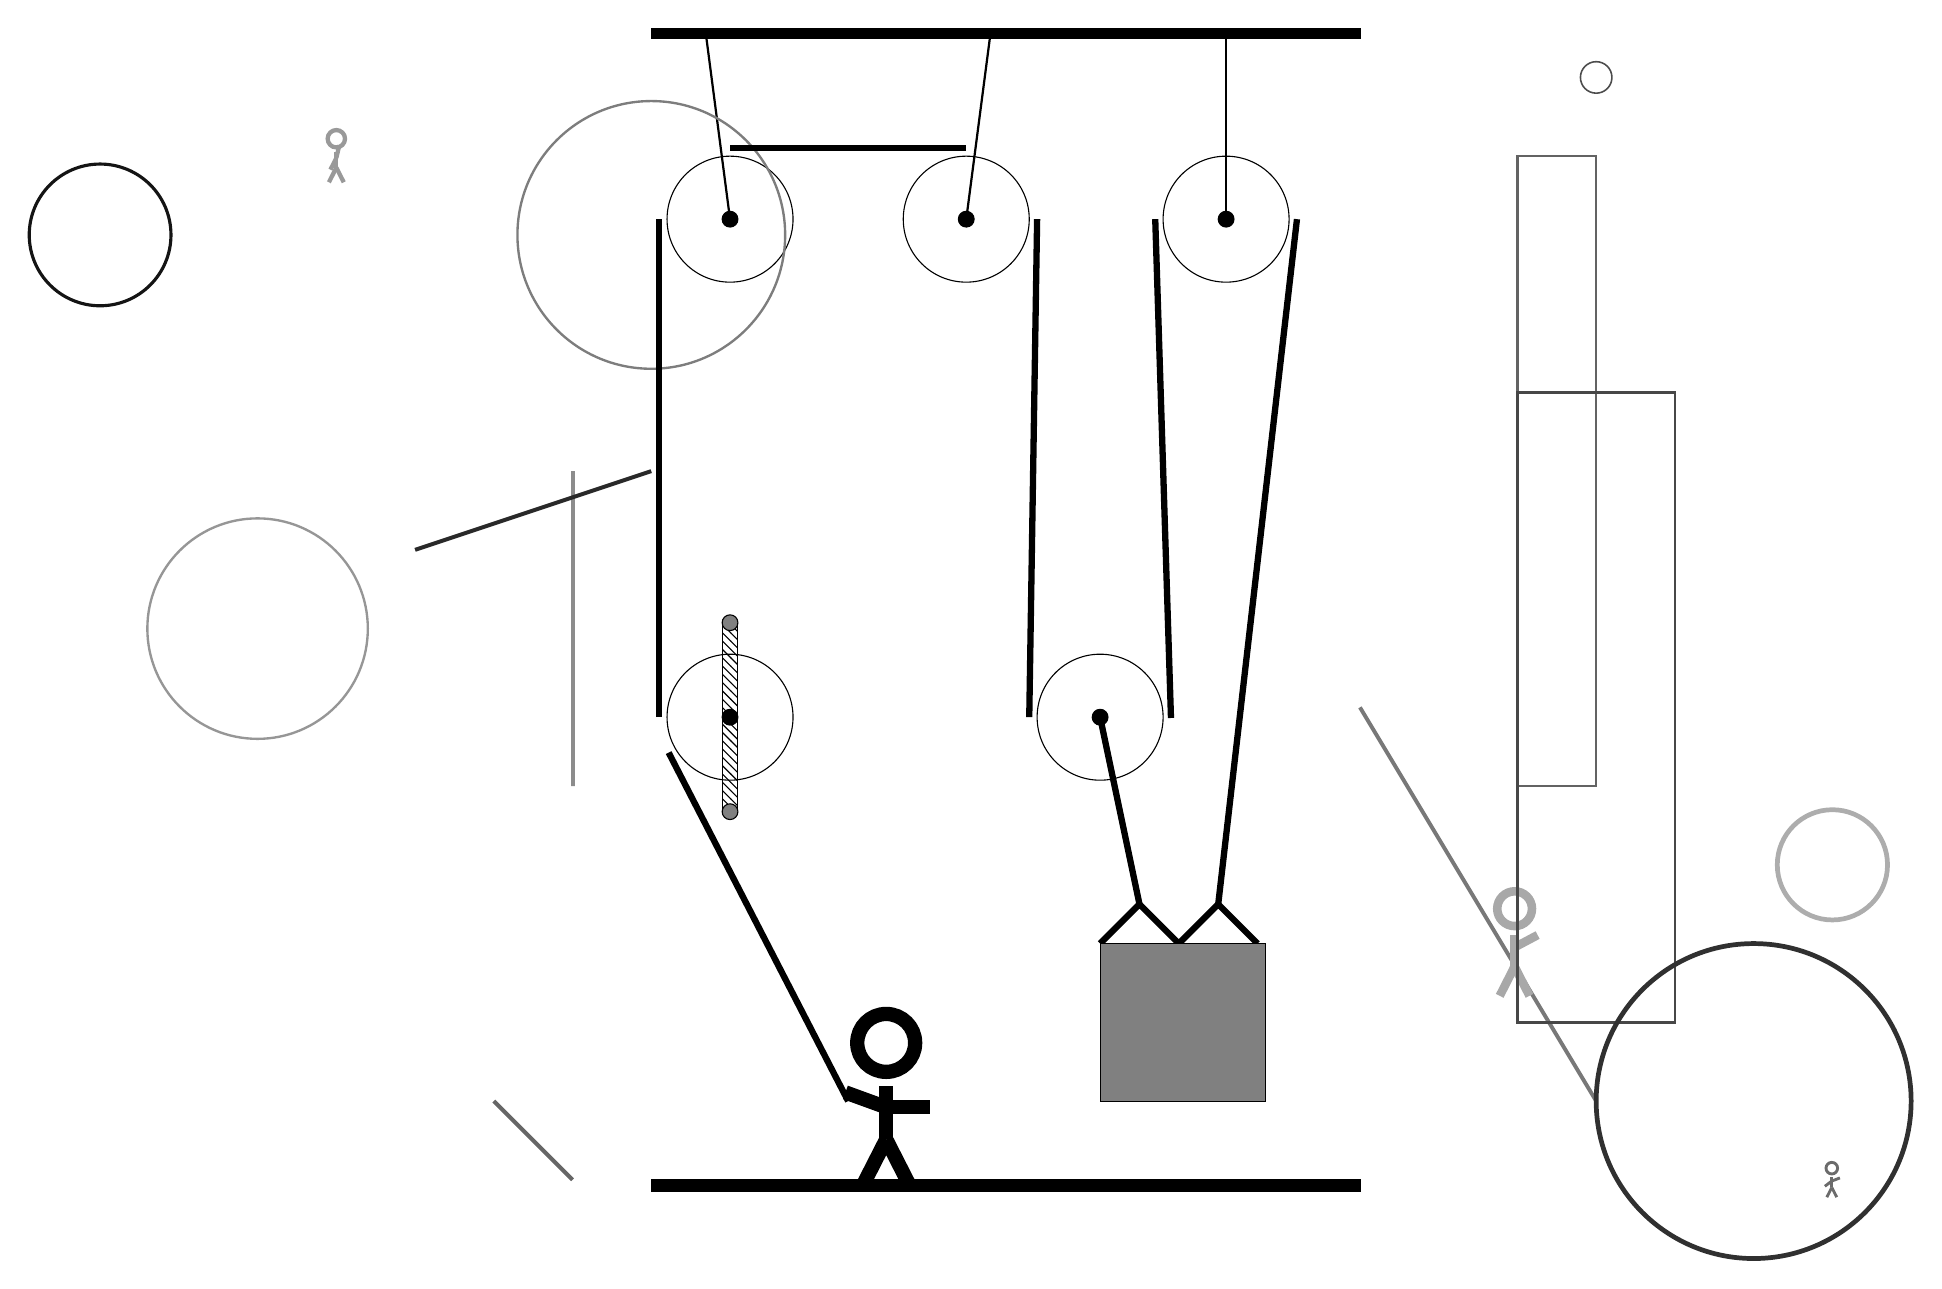
\begin{tikzpicture}
			%%%%% START %%%%%
			
			\draw[fill=black] (-3, 11.5) rectangle (6, 11.625);
			
			\draw (1, 9.2) circle (0.8);
			\draw[fill=black] (1, 9.2) circle (0.1);
			\draw[thick] (1, 9.2) -- (1.3, 11.5);
			
			\draw (4.3, 9.2) circle (0.8);
			\draw[fill=black] (4.3, 9.2) circle (0.1);
			\draw[thick] (4.3, 9.2) -- (4.3, 11.5);
			
			\draw (2.7, 2.875) circle (0.8);
			\draw[fill=black] (2.7, 2.875) circle (0.1);
			
			\draw[line width=0.8mm]  (2.7, 0.0) -- (3.2, 0.5) -- (3.7, 0.0) -- (4.2, 0.5) -- (4.7, 0.0);
			\draw[fill=black!50] (2.7, 0.0) rectangle (4.8, -2.0);
			
			\draw (-2, 9.2) circle (0.8);
			\draw[fill=black] (-2, 9.2) circle (0.1);
			\draw[thick] (-2, 9.2) -- (-2.3, 11.5);
			
			\draw (-2, 2.875) circle (0.8);
			\draw[fill=black] (-2, 2.875) circle (0.1);
			\draw[pattern=north west lines, pattern color=black] (-2.1, 4.075) rectangle (-1.9, 1.675);
			\draw[fill=black!50] (-2, 4.075) circle (0.1);
			\draw[fill=black!50] (-2, 1.675) circle (0.1);
			
			\draw[line width=0.5mm, color=black!45] (-4, 6) rectangle (-4, 2);
			
			\draw[line width=0.5mm, color=black!53](6, 3) -- (9, -2);
			\node[line width=0.7mm, color=black!58] at (12, -3) {\Strichmaxerl[2][37][21]};
			\draw[line width=0.5mm, color=black!60](-5, -2) -- (-4, -3);
			\draw [line width=0.6mm, color=black!32](12, 1) circle (0.7);
			\node[line width=0.2mm, color=black!34] at (8, 0) {\Strichmaxerl[6][89][28]};
			\draw[line width=0.3mm, color=black!61] (8, 10) rectangle (9, 2);
			
			\draw[line width=0.3mm, color=black!72] (8, -1) rectangle (10, 7);
			\draw[line width=0.5mm, color=black!84](-6, 5) -- (-3, 6);
			
			\draw [line width=0.3mm, color=black!41](-8, 4) circle (1.4);
			\draw [line width=0.3mm, color=black!51](-3, 9) circle (1.7);
			\draw [line width=0.6mm, color=black!81](11, -2) circle (2.0);
			\draw [line width=0.4mm, color=black!92](-10, 9) circle (0.9);
			
			\node[line width=0.7mm, color=black!40] at (-7, 10) {\Strichmaxerl[3][63][77]};
			\draw [line width=0.2mm, color=black!70](9, 11) circle (0.2);
			
			\draw[line width=0.8mm](-0.5, -2) -- (-2.7794, 2.425);
			\centerarc[line width=0.8mm](-2, 2.875)(180:210:0.9);
			\draw[line width=0.8mm](-2.9, 2.875) -- (-2.9, 9.2);
			\centerarc[line width=0.8mm](-2, 9.2)(90:180:0.9);
			
			\draw[line width=0.8mm](-2, 10.1) -- (1, 10.1);
			\centerarc[line width=0.8mm](1, 9.2)(0:90:0.9);
			\draw[line width=0.8mm](1.9, 9.2) -- (1.8, 2.875);
			\centerarc[line width=0.8mm](2.7, 2.875)(180:370:0.9);
			\draw[line width=0.8mm] (3.6, 2.865) -- (3.4, 9.2);
			\centerarc[line width=0.8mm](4.3, 9.2)(0:180:0.9);
			\draw[line width=0.8mm](4.2, 0.5) -- (5.2, 9.2);
			\draw[line width=0.8mm] (3.2, 0.5) -- (2.7, 2.875);
			
			\node at (0, -2) {\Strichmaxerl[10][-20][0]};
			
			\draw[fill=black] (-3, -3) rectangle (6, -3.15);
			
			%%%%% END %%%%%
		\end{tikzpicture}
	\end{figure}	
\end{document}